\chapter{Methodology}
This chapter delineates the methodological framework and engineering design choices utilized to implement the real-time person-following system. It translates the theoretical foundations and state-of-the-art concepts into a concrete architectural blueprint. The following sections outline the precise system requirements, detail the decentralized software-hardware architecture, and explain the algorithmic pipelines responsible for deep-learning-based perception, spatial localization, and robotic motion control.

\section{System Requirements}
To ensure the successful development and deployment of the person-following robot, a rigorous set of system requirements was defined. These criteria are categorized into functional requirements (FR), which dictate the core capabilities of the platform, and non-functional requirements (NFR), which establish the operational constraints and performance benchmarks.

\subsection{Functional Requirements}
\begin{itemize}
	\item \textbf{FR-1: Automated Human Detection:} The system must autonomously identify a human target within the camera's field of view utilizing deep learning object detection models.
	\item \textbf{FR-2: Real-Time Spatial Localization:} The robot must continuously calculate the relative 3D spatial coordinates (X, Y, Z) of the detected person using synchronized depth sensor data.
	\item \textbf{FR-3: Active Target Tracking:} The locomotive base must dynamically adjust its linear and angular velocities to follow the designated human target at a safe distance.
	\item \textbf{FR-4: Integrated Safety Interrupts:} The platform must process physical bumper collisions and emergency stop triggers to halt the actuators instantly, prioritizing user safety.
\end{itemize}

\subsection{Non-Functional Requirements}
\begin{itemize}
	\item \textbf{NFR-1: Low Latency Inference:} The entire perception-to-actuation pipeline must operate with minimal latency, targetting a real-time frame rate of at least 15 to 30 frames per second (FPS) on the edge device.
	\item \textbf{NFR-2: Computational Efficiency:} High-level deep learning tasks must not overload the central processing unit (Raspberry Pi 4), ensuring that critical robotic navigation services remain stable.
	\item \textbf{NFR-3: Modular Software Architecture:} The software components must be decoupled into independent ROS 2 nodes to ensure scalability, ease of debugging, and maintainability.
\end{itemize}

\section{Overall System Architecture}
The architectural design of the proposed system utilizes a distributed offloading paradigm due to the heavy computational demands of deep learning inference. Initial testing revealed that the onboard Raspberry Pi 4 Single-Board Computer (SBC) lacked the processing capabilities required to run the YOLO object detection pipeline at a responsive real-time frame rate. While the Luxonis OAK-D Pro camera features an integrated Visual Processing Unit (VPU) capable of edge computing, utilizing this onboard hardware was out of scope for the timeline of this thesis. 

Consequently, the physical framework is divided into a dedicated external computing unit and the mobile robot platform. The raw sensory data from the OAK-D Pro camera is passed directly through the Raspberry Pi 4 without local processing and transmitted over a local wireless network to an external workstation (laptop). This workstation serves as the primary processing hub, executing the high-level computer vision models, spatial localization, and state machine transitions. Communication and data synchronization between the external laptop and the TurtleBot 4 base are managed natively via the Eclipse CycloneDDS middleware, ensuring low-latency transport of control commands back to the iRobot Create 3 base actuators.


\section{Software Design}
The software architecture is designed around the principles of modularity and asynchronous communication inherent to ROS 2. Rather than relying on a single, monolithic executable, the system is divided into specialized, decoupled software components known as nodes. 

Communication between these nodes is achieved through standardized ROS 2 interfaces, specifically utilizing topics for high-frequency telemetry and actions for long-running, interruptible behaviors. To prevent data corruption or race conditions, the nodes utilize a language-agnostic data layout. This modular software design allows the system to remain highly robust; for instance, if the high-level perception pipeline experiences a momentary delay, the lower-level safety layers on the mobile base can still act independently to prevent collisions.

\subsection{Detection Pipeline}
The detection pipeline is responsible for extracting semantic meaning from raw environmental inputs. Instead of processing data locally on the camera hardware, it utilizes the YOLO architecture executing directly on the external laptop workstation. The raw, high-resolution RGB image stream captured by the OAK-D Pro sensor array is transmitted over the network and continuously downscaled on the host machine to match the specific input matrix dimensions required by the neural network.

\begin{figure}[!ht]
	\centering
	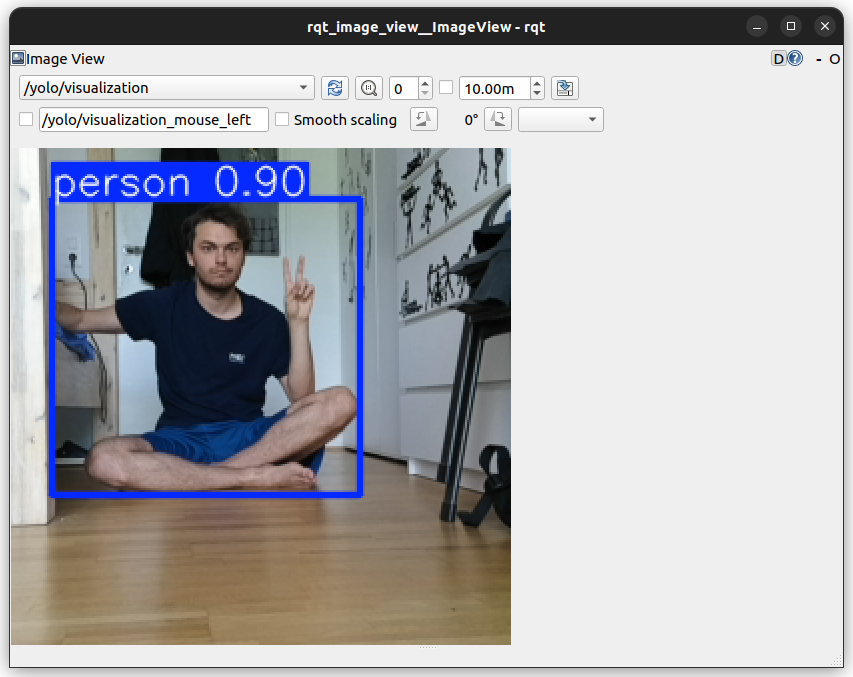
\includegraphics[width=0.8\linewidth]{figures/det_pipeline.png}
	\caption[Detection Pipeline]{Detection pipeline detecting a human}
	\label{fig:det_pipeline}
\end{figure}

The forward pass of the model, computed entirely by the workstation's graphics processor, generates boundary bounding boxes, class labels, and confidence scores for all detected entities within the frame. A specialized software filter is subsequently applied within the custom ROS 2 node to discard all classes except the "person" label. To minimize false positives and ensure stable tracking, a confidence threshold of $\tau \ge 0.8$ is enforced. The final output of this pipeline is a filtered 2D bounding box representing the precise horizontal and vertical pixel coordinates of the human target within the image plane, which is then made available for spatial localization.

\section{Object Localization}
Once the 2D bounding box of the human target is established, the object localization module maps these pixel coordinates into a 3D spatial coordinate frame relative to the robot. This is achieved by fusing the 2D vision data with the synchronized stereo depth map provided by the camera's global-shutter monochrome sensors.

\begin{figure}[!ht]
	\centering
	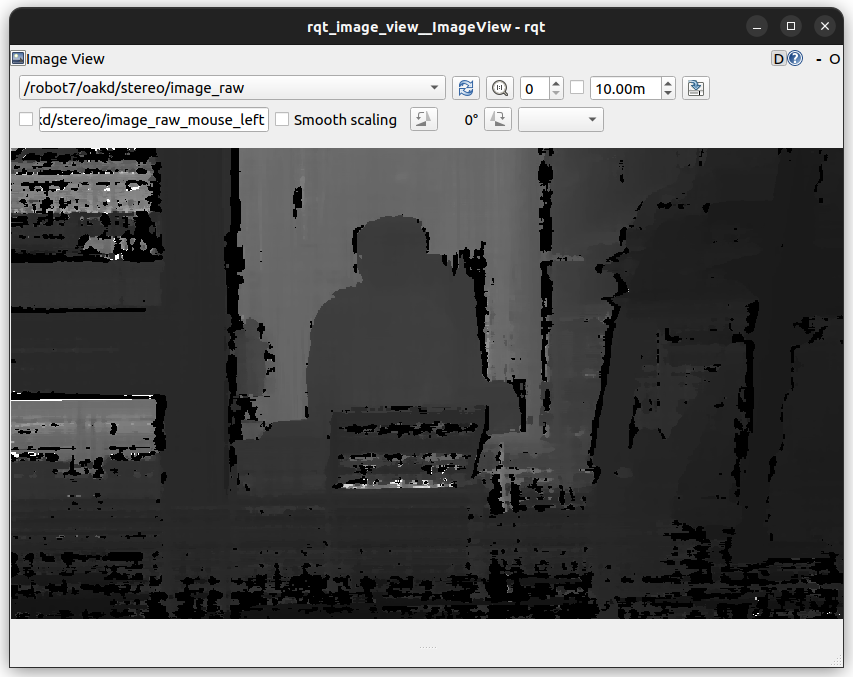
\includegraphics[width=0.8\linewidth]{figures/depth_image.png}
	\caption[Stereo depth image]{Stereo depth image}
	\label{fig:stereo_image}
\end{figure}

The algorithm calculates the region of interest (ROI) on the depth map that corresponds to the center of the 2D bounding box. By extracting the median depth value within this spatial patch, the system determines the absolute Euclidean distance ($Z$) along the camera's optical axis. Using the camera's intrinsic calibration parameters—specifically the focal length ($f_x, f_y$) and the optical center ($c_x, c_y$)—the system applies pixel-to-3D back-projection. This mathematical transformation yields the exact spatial coordinates $(X, Y, Z)$ of the target in meters, which are then continuously published as a standardized coordinate transform (TF2) tree within ROS 2.

\section{Person Following Strategy}
The locomotive strategy of the robot is governed by a Finite State Machine (FSM). This architectural choice ensures predictable and robust transitions between different operational phases based on the tracking status of the target. The logical flow and transition conditions between the individual states are illustrated in Figure~\ref{fig:fsm_transitions}.

\begin{figure}[!ht]
	\centering
	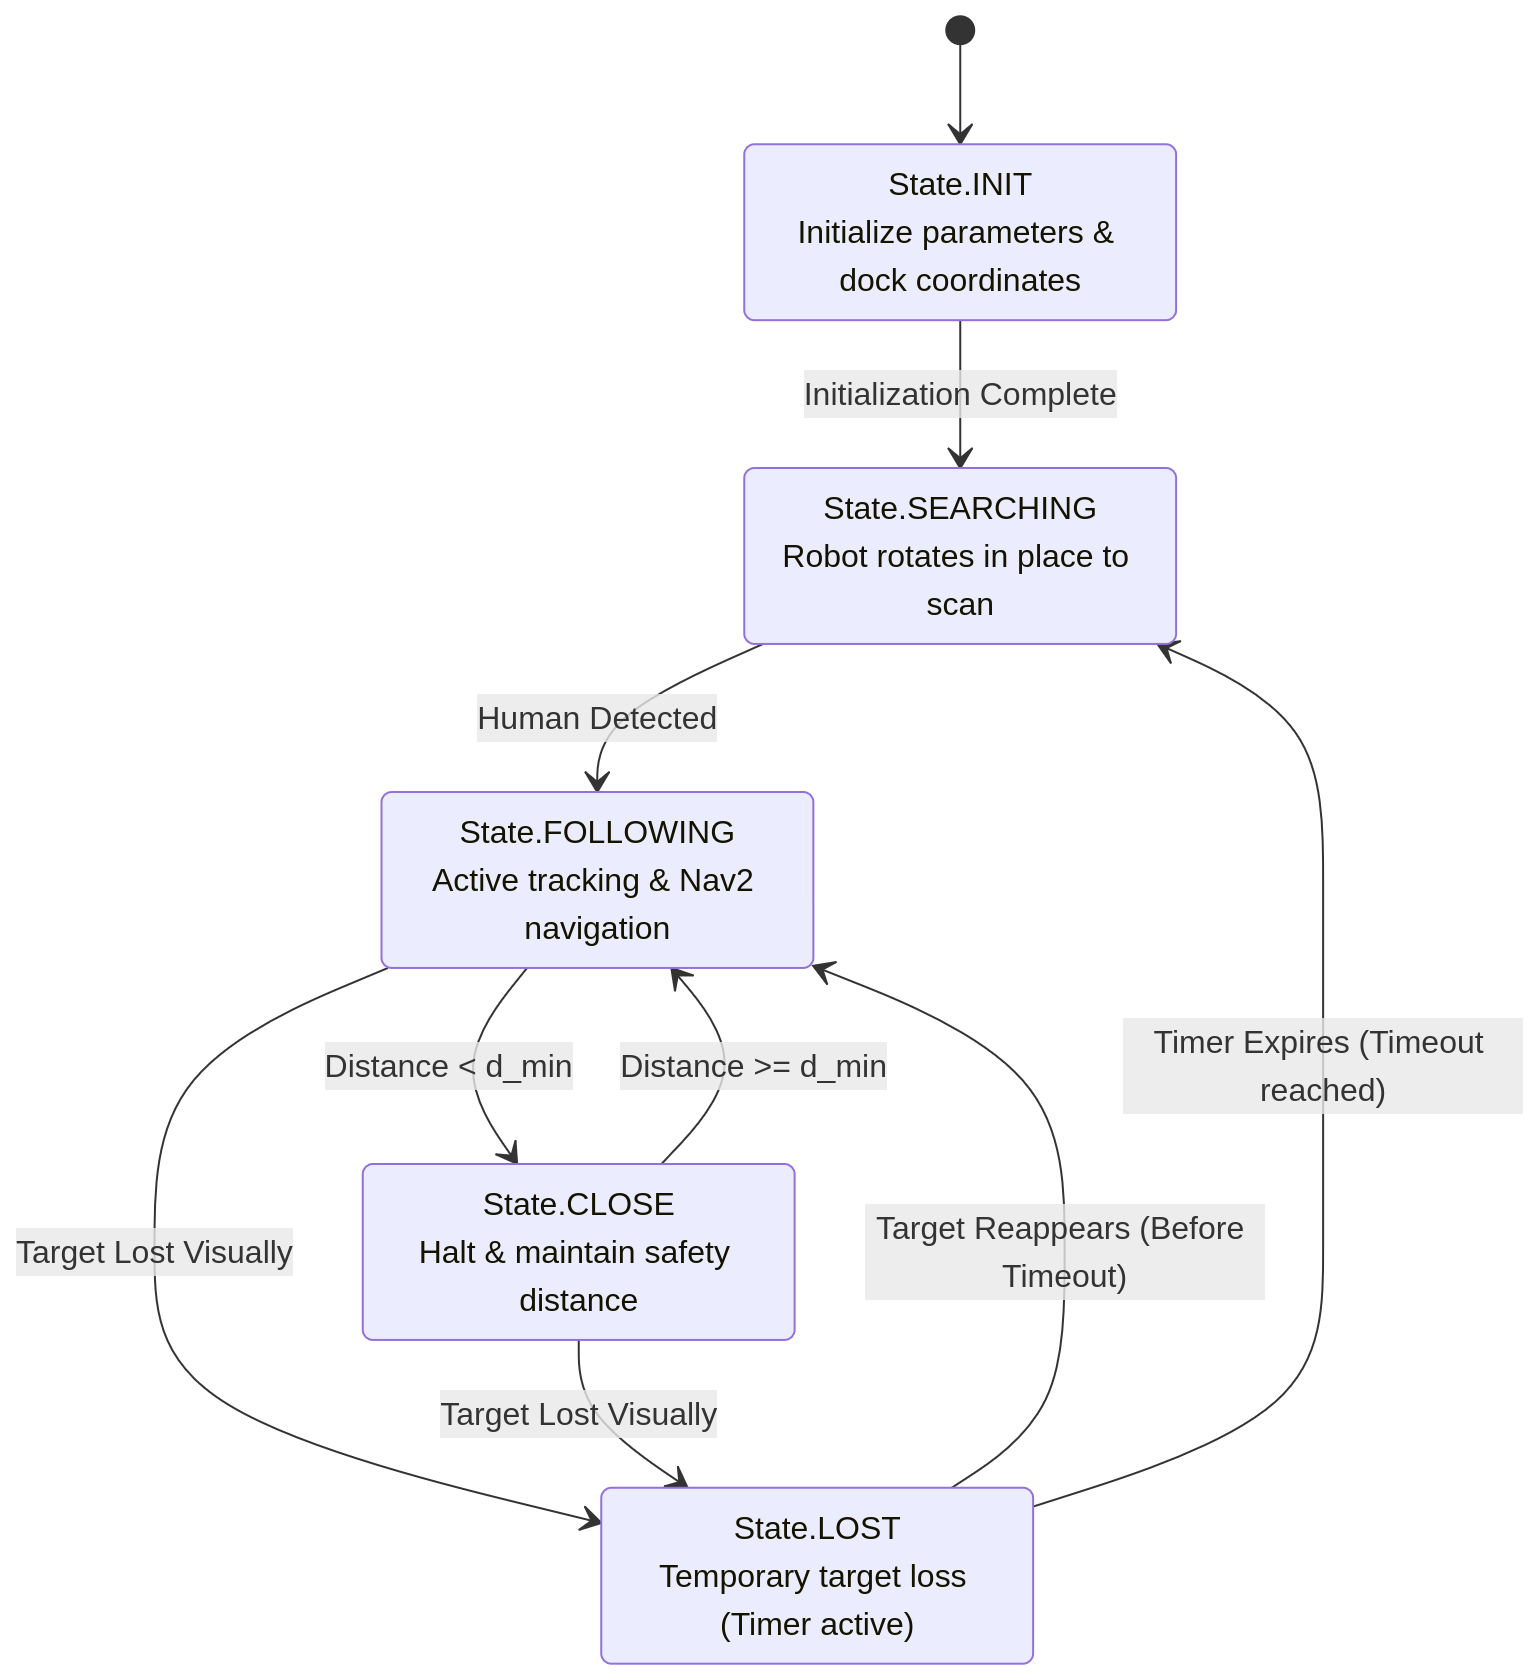
\includegraphics[width=0.8\linewidth]{figures/state_machine.png}
	\caption[Finite State Machine Transition Diagram]{State transition diagram of the centralized controller, highlighting the operational logic from initialization to target loss handling.}
	\label{fig:fsm_transitions}
\end{figure}

\newpage

The FSM consists of five distinct states:

\begin{itemize}
	\item \textbf{\texttt{State.INIT}:} The initialization phase where essential baseline parameters and starting conditions are established, such as capturing the robot's initial position while docked at the charging station.
	\item \textbf{\texttt{State.SEARCHING}:} Triggered when no human target is visible. In this state, the robot executes a continuous, controlled rotation in place to scan its surroundings and locate a person.
	\item \textbf{\texttt{State.FOLLOWING}:} The active tracking state. The robot computes the distance and angle to the detected human and follows them smoothly until the target either enters the safety zone or is visually lost.
	\item \textbf{\texttt{State.CLOSE}:} A safety-enforcement state activated when the human target is within close proximity. The TurtleBot 4 stops its translational movement to maintain a strict predefined safety distance from the person.
	\item \textbf{\texttt{State.LOST}:} A temporary transitional state entered immediately when the person disappears from the camera's field of view. A software timer is initiated upon entering this state. If the target reappears within the image frame before the timer expires, the FSM transitions smoothly back to \texttt{State.FOLLOWING}. If the timer running out confirms the target is permanently lost, the robot reverts to \texttt{State.SEARCHING}.
\end{itemize}
